%%%%%%%%%%%%%%%%%%%%%%%%%%%%%%%%%%%%%%%%%%%%%%%%%%%%%%%%%%%%%%%%%
% Tese de Doutorado / Dept. Fisica, CFM, UFSC                   %
% Lacerda@CórregoGrande - Jan/2018                              %
%%%%%%%%%%%%%%%%%%%%%%%%%%%%%%%%%%%%%%%%%%%%%%%%%%%%%%%%%%%%%%%%%

%:::::::::::::::::::::::::::::::::::::::::::::::::::::::::::::::%
%                                                               %
%                          Capítulo 4                           %
%                                                               %
%:::::::::::::::::::::::::::::::::::::::::::::::::::::::::::::::%

%***************************************************************%
%                                                               %
%                        DIG discussion                         %
%                                                               %
%***************************************************************%

\chapter{Discussão}
\label{sec:DIGdisc}
Nosso método de classificação é inspirado em argumentos teóricos e empíricos possui diversos propósitos. Neste capítulo vamos aplicar nosso méotodo para nossa amostra do CALIFA cobrindo alguns objetivos específicos:
\begin{enumerate*}[label=(\roman*)]
    \item estimar a relevância do hDIG, mDIG e SFc sobre galáxias cobrindo toda a sequência de Hubble;
    \item estudar a natureza da emissão difusa extraplanar nos sistemas {\em edge-on};
    \item comparar resultados obtidos com o nosso método frente aqueles que separam SF/DIG baseados em um limite fixo em $\Sigma_{\Ha}$;
    \item investigar a possibilidade de discernimento entre regimes DIG e SF baseados em razões de linhas sensíveis à densidade do meio;
    \item testar a consistência de nosso sistema de classificação analisando através de um diagrama clássico de linhas de emissão;
    \item examinar a mistura presente no mDIG;
    \item fechamos a discussão com os possíveis adversidades em nosso estudo.
\end{enumerate*}

\section{A relevância das componentes hDIG, mDIG e SFc}
\label{sec:DIGdisc:relstrenghts}

%---------------------------- Figure ----------------------------
\begin{figure}
 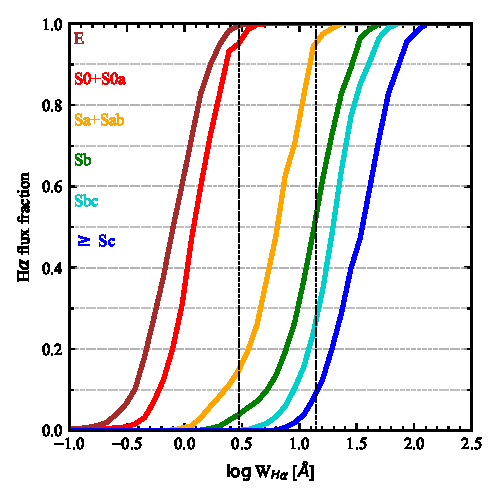
\includegraphics{figuras/fig_cumul_fHaWHa_per_morftype.pdf}
 \caption[Fração cumulativa do fluxo de ${\rm H}\alpha$ com o crescimento de $W_{{\rm H}\alpha}$ para diferentes classes morfológicas]
 {Fração cumulativa do fluxo total de \Ha provenientes de regiões com $W_{\Ha}$ menor que determinado valor. O gráfico mostra as curvas medianas obtidas para galáxias presentes em cada uma de nossas seis classes morfológicas.}
 \label{fig:CurveOfGrowth}
\end{figure}
%---------------------------- Figure ----------------------------

Dentre as questões que podemos perscrutar neste estudo, a importância relativa das componentes de nossa classificação talvez seja a mais importante. A dominância e a evolução da influência que cada um dessas componentes tem sobre galáxias através de diferentes tipos morfológicos é importante na interpretação de propriedades derivadas de dados espectrais não resolvidos espacialmentes. Nesses estudos as assinaturas de regimes distintos vêm todas misturadas sob o mesmo espectro.

Uma maneira simples e relevante observacionalmente de quantificar isso é calculando a contribuição relativa de cada componente para o fluxo total de \Ha. Por exemplo, nas galáxias na Figura \ref{fig:ExampleMaps} essas frações vão de $(f_{\rm hDIG} , f_{\rm mDIG} , f_{\rm SFc}) = (87,13,0)$ para a galáxia S0 CALIFA 0072, até $(5.5,47,47.5)$ para a galáxias Sb CALIFA 0010, e $(0.3,46.1,53.6)$ para a CALIFA 0813, uma Sbc. Essa progressão ao longo da sequência de Hubble reflete as tendências que podem ser vistas na Figure \ref{fig:WHaDistrib_ALLgals}. No canto superior direito de cada painel temos os valores de $(f_{\rm hDIG} , f_{\rm mDIG} , f_{\rm SFc})$ para diferentes distâncias radiais e diferentes tipos morfológicos.

De maneira mais elaborada, a Figura \ref{fig:CurveOfGrowth} mostra essas frações para toda a amostra através dos valores medianos de cada classe morfológica. Nós calculamos a fração cumulativa do fluxo de \Ha, $f$, proveniente de regiões que possuem $W_{\Ha}$ menor que determinado valor. As curvas de $f(<W_{\Ha})$ representam como a fração cumulativa cresce com relação a $W_{\Ha}$. Na figura mostramos as curvas medianas para as nossas seis classes morfológicas. As linhas tracejadas verticais representam nossas fronteiras hDIG/mDIG e mDIG/SFc, em 3 e 14 \AA\ respectivamente.

A progressão constante de {\em early-} para {\em late-type} nessas curvas confirmam nossas expectativas provenientes das distribuições de $W_{\Ha}$ (Figura \ref{fig:WHaDistrib_ALLgals}) além de também nos permitir quantificar a importância relativa entre as componentes e o fluxo total de \Ha. Em galáxias elípticas ou S0 temos praticamente toda a emissão de \Ha na fase hDIG ($W_{\Ha} \le 3$). Entre os sistemas Sa-Sab, essa componente se encarrega por 14\% do fluxo de \Ha, com o mDIG sendo o responsável por praticamente todo o fluxo restante. De Sb para frente, o regime SFc domina, sendo responsável por 50\% ou mais. Natualmente existe um espalhamento natural nos dados, mesmo quando divididos em classes morfológicas.

A contribuição relativa do DIG para a emissão em \Ha foi estimada em diversos estudos anteriores, geralmente baseados em dados obtidos com filtros estreitos (\Ha + \nii) \citep{Ferguson.etal.1996, Zurita.etal.2000, Thilker.etal.2002, Oey.etal.2007}, com resultados variando substancialmente principalmente devido a diferenças na metodologia de separação da emissão difusa. O maior estudo até hoje foi feito por \citet{Oey.etal.2007}, que estimaram a fração de emissão difusa em \Ha de $59\pm19 \%$ sobre uma amostra de 109 galáxias do {\em survey} SINGG \citep{Meurer.etal.2006}. Para nossa amostra (e nossas definições) nós encontramos um valor bem próximo, 56\% (hDIG + mDIG), mas com um espalhamento muito maior, $\pm38 \%$. Diferentemente de nosso estudo (Figura \ref{fig:CurveOfGrowth}), eles não encontraram nenhuma evidencia de correlação com o tipo morfológico. Talvez o motivo seja devido a diferença de critério e metodologia de classificação DIG/SF.


\section{Emissão extraplanar em sistemas {\em edge-on}}
\label{sec:DIGdisc:edgeon}

%---------------------------- Figure ----------------------------
\begin{figure}
 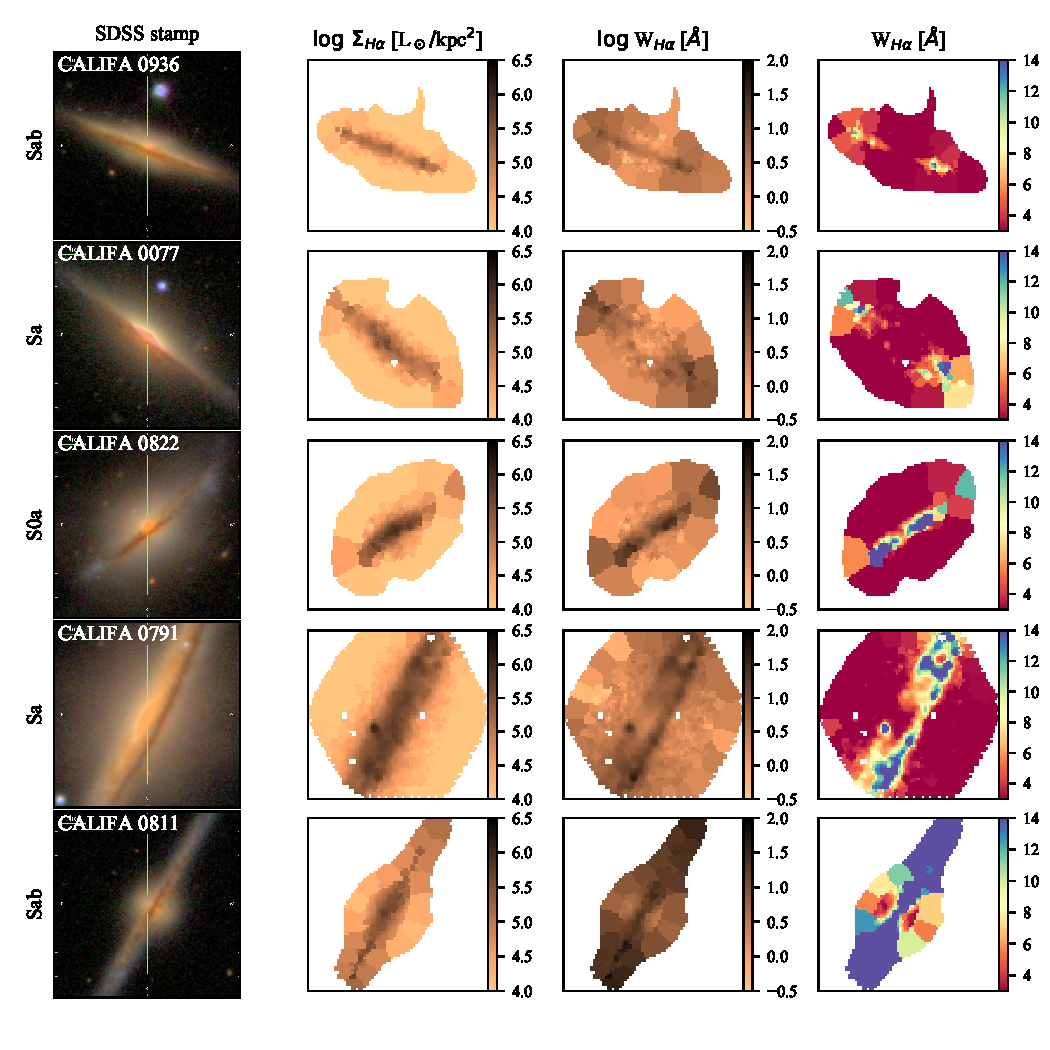
\includegraphics{figuras/fig_maps_class_edgeon_paper.pdf}
 \caption[Imagem \SDSS e mapas de $\Sigma_{{\rm H}\alpha}$ e $W_{{\rm H}\alpha}$: sistemas {\em edge-on}]
 {Como a Figura.\ \ref{fig:ExampleMaps}, mas para galáxias {\em edge-on}.}
 \label{fig:ExampleMapsEdgeOn}
\end{figure}
%---------------------------- Figure ----------------------------

Devido ao comportamento sistemático das propriedades de linhas de emissão, esses sistemas altamente inclinados são importantes para o estudo da emissão DIG nas regiões acima (e abaixo) do disco galáctico \citep{Tullmann.and.Dettmar.2000, Otte.etal.2002, Jones.etal.2017}. A galáxia protótipo utilizada nesses estudos é a NGC 891, extensivamente observada em diversos comprimentos de onda \citep{Rand.1998, Hodges.and.Bregman.2013, Seon.etal.2014, Hughes.etal.2015}. Esses estudos enfatizaram que as propriedades de linhas de emissão observadas no DIG extraplanar não podem ser explicadas puramente por fótons Lyman que escapam de regiões \hii presentes no disco. Uma variedade de fenômenos que pudessem gerar tal emissão foram sugeridos, como: dissipação de turbulência \citep{Minter.and.Spangler.1997}, reconexão magnética \citep{Raymond.1992}, choques \citep{Collins.and.Rand.2001}, raios cósmicos, aquecimento fotoelétrico proveniente de grãos de poeira do meio interestelar  \citep{Weingartner.and.Draine.2001}, e fótons Lyman vindos de estrelas velhas e quentes \citep{FloresFajardo.etal.2011a}.

A Figura \ref{fig:ExampleMapsEdgeOn} nos mostra como os dados do CALIFA podem nos trazer um novo {\em insight} ao problema. Nela vemos cinco exemplos de galáxias {\em edge-on} dispostas da mesma forma que na Figura \ref{fig:ExampleMaps}. As quatro primeira possuem configuração muito parecida, onde temos o disco e arredores dominados por mDIG e SFc, enquanto a grandes distâncias do disco galácticos vemos uma completo predomínio de hDIG. Isso favorece o cenário proposto por \citet{FloresFajardo.eteal.2011a}, onde a ionização se torna dominada por HOLMES à medida que nos afastamos do plano galáctico. Essa conclusão é reforçada pelos mapas de diagnóstico de razões de linhas baseados em dados do MaNGA em \citet{Belfiore.etal.2016} e \citet{Zhang.etal.2017a}.

Através de nossa experiência calculando $\xi$ (veja a Seção \ref{sec:DIGclass:WHaDistrib_hDIG}) podemos, pela primeira vez, relacionar a emissão DIG extraplanar com as populações estelares subjacentes. A mediana de $\xi$ nas regiões extraplanares das quatro primeiras galáxias na Figura \ref{fig:ExampleMapsEdgeOn} é 1.5 com interquartis 1.1--1.9. Dado um fator de $2 \sim 3$ nessa estimativa \citep{CidFernandes.etal.2011a} a conclusão principal aqui é que $\xi$ é da ordem de 1 e por isso consegue produzir fótons com $h\nu > 13.6$ suficientes para explicar a emissão extraplanar de \Ha.

Se essas galáxias fossem vistas {\em face-on}, o DIG extraplanar estaria projetado por cima do disco, que é dominado por mDIG + SFC. Para uma emissividade constante de \Ha, a razão entre $\Sigma_{\Ha}$ {\em face-on} e {\em edge-on} é igual a razão entre $h/r$ (altura e raio) da camada hDIG extraplanar. Nas galáxias da Figura \ref{fig:ExampleMapsEdgeOn} o valor de $\Sigma_{\Ha}$ é de aproximadamente algumas vezes $10^4 L_\odot\,$kpc$^{-2}$. Para $h \sim r$, este também deve ser o brilho superficial dessa componente. Esse valor é muito menor que os que estão presentes nas regiões SFc das galáxias {\em face-on} da Figura \ref{fig:ExampleMaps}, nesse caso, portanto, o efeito do hDIG extraplanar projetado pode ser negligenciado. Porém, algumas regiões mDIG apresentam valores não muito maiores que $10^4 L_\odot\,$kpc$^{-2}$ podendo assim carregar alguma contribuição não-negligenciável do hDIG extraplanar.

A galáxia na última linha da Figura \ref{fig:ExampleMapsEdgeOn} (CALIFA 0811, UGC 10043) é diferente das demais, como podemos ver pelo seu mapa de classificação. Ela possui muito mais SFc no seu disco e em regiões extraplanares, além de um cone bipolar com valores intermediários de $W_{\Ha}$ centrado no núcleo. Essa galáxia foi recentemente estudada por \citet{LopezCoba.etal.2017}, no qual encontraram razões entre linhas de emissão e cinemática consistentes com vento galáctico alimentado por um evento SF central. Essa combinação de ionização por choque e formação estelar espalhada pelo disco explica porque não há emissão hDIG extraplanar nessa galáxia, embora seja curioso que os valores de $W_{\Ha}$ caiam para valores hDIG nas partes internas do bicone.


\section{Comparações com esquemas de separação SF/DIG baseados em $\Sigma_{{\rm H}\alpha}$}
\label{sec:DIGdisc:compSBHa}

%---------------------------- Figure ----------------------------
\begin{figure}
 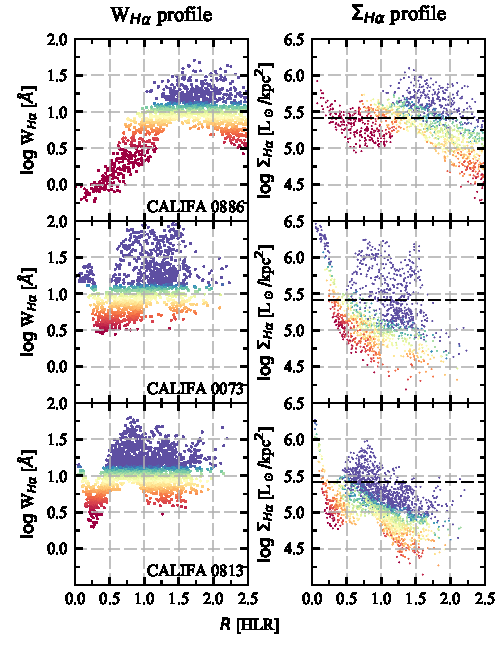
\includegraphics[scale=1.7]{figuras/fig_WHaSBHa_profile_faceon_paper.pdf}
 \caption[Perfis radiais de $W_{{\rm Ha}\alpha}$ e $\Sigma_{{\rm Ha}\alpha}$]
 {Perfis radiais de $W_{{\rm Ha}\alpha}$ e $\Sigma_{{\rm Ha}\alpha}$ para três galáxias presentes na Figura \ref{fig:ExampleMaps}. Os pontos são coloridos segundo $W_{\Ha}$. As linhas pontilhadas nos painéis da direita marcam $\Sigma_{\Ha} = 10^{39}$ erg$\,$s$^{-1}\,$kpc$^{-2}$.}
 \label{fig:WHa_and_SHa_profiles}
\end{figure}
%---------------------------- Figure ----------------------------

Apesar das vantagens conceituais desse modo de classificação apresentado até agora, $W_{\Ha}$ possui $\Sigma_{\Ha}$ no seu numerador, por isso pode-se imaginar que um modelo de classificação baseado nessas duas variáveis deveriam ter resultados semelhantes. Através dos mapas da Figura \ref{fig:ExampleMaps} podemos perceber que algumas estruturas, como os braços de formação estelar, são concomitantemente identificados por $W_{\Ha}$ e $\Sigma_{\Ha}$, porém outras não são. Mais precisamente, $\Sigma_{\Ha}$ sempre tem um máximo no centro da galáxia, porém, para galáxias {\em early-type}, $W_{\Ha}$ mostra evidentes declives.

Três exemplos de galáxias presentes na Figura \ref{fig:ExampleMaps}, CALIFA 0886, 0073 e 0813, com seus respectivos perfis radiais de $W_{\Ha}$ e $\Sigma_{\Ha}$ aparecem na Figura \ref{fig:WHa_and_SHa_profiles}. (Exemplos de perfis radiais como esses podem ser encontrados em \citealt{Papaderos.etal.2013, Belfiore.etal.2016, Belfiore.etal.2017, Gomes.etal.2016b, GonzalezDelgado.etal.2016a}.) Na coluna da esquerda (direita) temos os valores de $W_{\Ha}$ ($\Sigma_{\Ha}$) contra R. Ambos são coloridos por $W_{\Ha}$ segundo o mesmo esquema de cores utilizado até aqui.

A CALIFA 0886 é um bom exemplo de galáxia que apresenta valores baixos de $W_{\Ha}$ em seu centro dominado por emissão hDIG, porém com um pico em $\Sigma_{\Ha}$ nessa mesma região. A alta concentração de HOLMES no bojo da galáxia faz com que o mesmo seja muito mais brilhante que o disco que o cinge. O aumento do brilho superficial de \Ha devido a geometria do bojo pode fazer com que essa emissão seja incorretamente classificada como SF quando utilizamos um esquema de classificação SF/DIG baseados em $\Sigma_{\Ha}$. Como vemos no painel do topo à direita, os valores de $\Sigma_{\Ha}$ estão acima da linha pontilhada, que marca o limite que seleciona confiávelmente spaxels dominados por regiões \hii segundo \citet{Zhang.etal.2017a}, $\Sigma^{\rm SF,min}_{\Ha} = 10^{39}$ erg$\,$s$^{-1}\,$kpc$^{-2} =  2.6 \times 10^{5} L_\odot\,$kpc$^{-2}$. No entanto, vemos que as mesmas regiões possuem $W_{\Ha} \sim 1$ \AA, sem dúvidas operando sob regime hDIG. O critério utilizando $W_{\Ha}$ corretamente classifica o bojo dessa e de outras galáxias como aposentado, enquato um critério baseado em $\Sigma_{\Ha}$ os interpretaria como dominados por regiões SF.

%---------------------------- Figure ----------------------------
\begin{figure}
 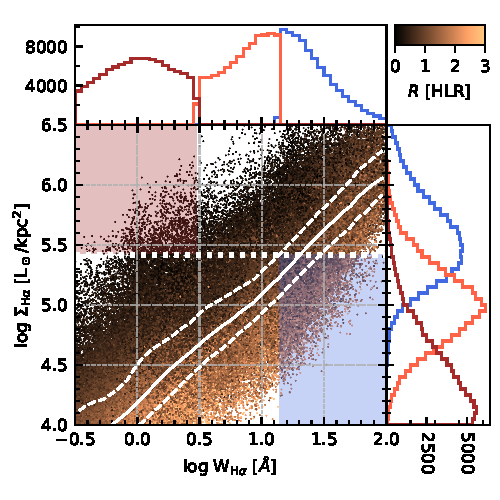
\includegraphics[scale=1.5]{figuras/fig_logSBHa_logWHa_histograms.pdf}
 \caption[$\log {\rm H}\alpha \times \log \Sigma_{{\rm H}\alpha}$]
 {$\log \Sigma_{\Ha}$ em função de $W_{\Ha}$ para as zonas de nossa amostra. Os intervalos em ambos eixos estão limitados àqueles valores que utilizamos para saturar os mapas na Figura \ref{fig:ExampleMaps}. Os pontos estão coloridos conforme a distânciada até o núcleo (em unidades de HLR). Os histogramas de $\Sigma_{\Ha}$ e de $W_{\Ha}$ estão coloridos com as mesmas cores utilizadas naqueles na Figura \ref{fig:WHa-Xi}. A linha contínua e as linhas tracejadas em branco marcam a mediana e o intervalo interquartil respectivamente. O limite $\Sigma^{\rm SF,min}_{\Ha} = 10^{39}$ erg$\,$s$^{-1}\,$kpc$^{-2}$ proposto por \citet{Zhang.etal.2017a} é sinalizando utilizando uma linha horizontal pontilhada branca. Um retângulo vermelho com bolas representa regiões classificadas como hDIG que possuem brilho superficial acima desse limite. Já aquelas regiões classificadas como SFc abaixo desse limite estão sobre um retângulo azul com estrelas.}
 \label{fig:logWHa_logSBHa_histo}
\end{figure}
%---------------------------- Figure ----------------------------

Ao longo do disco da CALIFA 0886 a classificação utilizando o limite proposto por \citet{Zhang.etal.2017a} em $\Sigma_{\Ha}$ concorda com o regime nebular identificado por $W_{\Ha}$. Essa concordância ocorre apenas de forma parcial na CALIFA 0073 (painéis centrais na Figura \ref{fig:WHa_and_SHa_profiles}), onde encontramos mais regiões SF no disco utilizando o critério baseado em $W_{\Ha}$ do que aquele em $\Sigma_{\Ha}$. Esse fato é ainda mais acentuado na CALIFA 0813 (painéis inferiores), onde a maioria das regiões com $W_{\Ha} > 14$ \AA\ possuem $\Sigma_{\Ha}$ abaixo do limite $\Sigma^{\rm SF,min}_{\Ha}$. Essas diferenças se originam nos comportamentos radiais distindos entre $\Sigma_{\Ha}$ e $W_{\Ha}$.

Na Figura \ref{fig:logWHa_logSBHa_histo} podemos ver tudo isso de forma estatística. Os pontos representam as zonas em nossa amostra, coloridos por $R$. Vemos que para um valor de $W_{\Ha}$, as regiões mais brilhantes (maior $\Sigma_{\Ha}$) estão localizadas nas regiões centrais. Já para um valor fixo de $\Sigma_{\Ha}$, os maiores valores de $W_{\Ha}$ tendem a estar nos arredores. De fato, como vimos nos exemplos da Figura \ref{fig:WHa_and_SHa_profiles}, $\Sigma_{\Ha}$ tende a diminuir enquanto $W_{\Ha}$ se mantém mais ou menos constante, ambos com grandes dispersões em qualquer $R$ no disco. Cerca de 37\% das nossas regiões SFcc possuem $\Sigma_{\Ha} < 10^{39}$ erg$\,$s$^{-1}\,$kpc$^{-2}$. Na média, essas regiões SFc pouco brilhantes estão localizadas em $R = 1.3$ HLR.

A área pintada em azul com estrelas na Figura \ref{fig:logWHa_logSBHa_histo} marca regiões em que $\Sigma_{\Ha} < \Sigma^{\rm SF,min}_{\Ha}$, porém com $W_{\Ha} > 14$ \AA, como vemos nos discos da CALIFA 0073 e na 0813. Se apoiando no exemplo da CALIFA 0886, vemos na área vermelha com bolas, regiões que seriam classificadas erroneamente utilizando o limite baseado em $\Sigma_{\Ha}$ proposto por \citet{Zhang.etal.2017a}. Também podemos ver nessas áreas pintadas, agora com relevância estatística, esses casos onde regiões SFc com baixo brilho nas estão geralmente situadas nas regiões exteriores e regiões dominadas pelo regime hDIG, porém muito brilhantes, situadas em $R < 1$.

Em resumo, comparado com o método de classificação em hDIG/mDIG/SFc baseado em $W_{\Ha}$ proposto neste trabalho, um critério baseado em $\Sigma_{\Ha}$ tente a sobrestimar a população de regiões SF situadas nas regiões mais internas das galáxias. De maneira mais critica, como já foi mencionado, $\Sigma_{\Ha}$ não pode, por si, identificar a componente hDIG, maior fonte de emissão em \Ha em velhos esferóides. Realmente temos visto que bojos aposentados ({\em retired bulges}) muitas vezes são classificados como SFc quando o brilho excede $\Sigma^{\rm SF,min}_{\Ha}$.

Trabalhos anteriores de utilizando dados do CALIFA por \citet{Kehrig.etal.2012}, \citet{Singh.etal.2013}, e \citet{Gomes.etal.2016b} também encontram valores $\Sigma_{\Ha}$, acima do limite $\Sigma^{\rm SF,min}_{\Ha}$ proposto por \citet{Zhang.etal.2017a}, nas regiões internas de galáxias {\em early-type}, onde incontestavelmente existe a ausência de estrelas jovens. (Veja também \citealt{Sarzi.etal.2010} para resultados baseados nos dados do SAURON\footnote{\em Spectrographic Area Unit for Research on Optical Nebulae survey}). Esses exemplos são realizações observacionais da inconsistência conceitual da soma de regiões DIG resultar em uma errônea classificação SF, apontada na Seção \ref{sec:DIGclass:WHaDistrib_hDIG}. O esquema apresentado nesta tese resolve esse problema extendendo para uma análise espacialmente resolvida, o conceito de galáxias aposentadas proposta por \citet{Stasinska.etal.2008a} e \citet{CidFernandes.etal.2011a} no contexto de espectros integrados.


\section{O DIG pode ser identificado por razões de linha sensíveis à densidade do meio?}
\label{sec:DIGdisc:nSii}

%% End of this chapter
